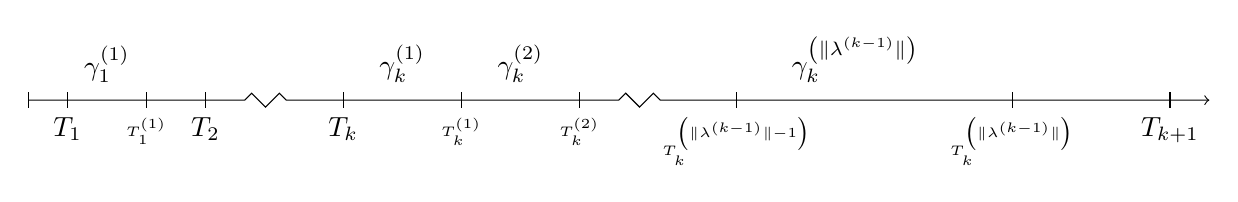
\begin{tikzpicture}
  \draw[->,decoration=zigzag] (0,0) -- (2.75, 0) decorate {--(3.4, 0)} --(7.5,0) decorate {--(8.15,0)}-- (15,0);
  % \draw[thick] (1,0) -- (2,0);
  % \draw[thick] (4.25,0) -- (7.25,0);
  \foreach \i in {0,.5,1.5,2.25,4,5.5,7,9, 12.5, 14.5} % numbers on line
  {
    \draw (\i,0.1) -- + (0,-0.2) ;
  }
  \node[below] at (.5,-.1) {$T_1$};
    \node[above] at (1,.1) {$\gamma_1^{(1)}$};
    \node[below] at (1.5,-.1) {\tiny$T_1^{(1)}$};
  \node[below] at (2.25,-.1) {$T_2$};

  \node[below] at (4,-.1) {$T_k$};
    \node[above] at (4.75,.1) {$\gamma_k^{(1)}$};
    \node[below] at (5.5,-.1) {\tiny$T_k^{(1)}$};
    \node[above] at (6.25,.1) {$\gamma_k^{(2)}$};
    \node[below] at (7,-.1) {\tiny$T_k^{(2)}$};

    \node[below] at (9,-.1){\tiny$T_k^{\left(\|\lambda^{(k-1)}\|-1\right)}$};
    \node[above] at (10.5,.1) {$\gamma_k^{\left(\|\lambda^{(k-1)}\|\right)}$};
    \node[below] at (12.5,-.1) {\tiny$T_k^{\left(\|\lambda^{(k-1)}\|\right)}$};


  \node[below] at (14.5,-.1) {$T_{k+1}$};
\end{tikzpicture}